\documentclass[12pt]{exam}

% essential packages
\usepackage{fullpage} % margin formatting
\usepackage{enumitem} % configure enumerate and itemize
\usepackage{amsmath, amsfonts, amssymb, mathtools} % math symbols
\usepackage{xcolor, colortbl} % colors, including in tables
\usepackage{makecell} % thicker \Xhline in table
\usepackage{graphicx} % images, resizing

% sometimes needed packages
\usepackage{hyperref} % hyperlinks
% \hypersetup{colorlinks=true, urlcolor=blue}
% \usepackage{logicproof} % natural deduction
% \usepackage{tikz} % drawing graphs
% \usetikzlibrary{positioning}
% \usepackage{multicol}
% \usepackage{algpseudocode} % pseudocode

% paragraph formatting
\setlength{\parskip}{6pt}
\setlength{\parindent}{0cm}

% newline after Solution:
\renewcommand{\solutiontitle}{\noindent\textbf{Solution:}\par\noindent}

% less space before itemize/enumerate
\setlist{topsep=0pt}

% creates \filcl to grey out cells for groupwork grading
\newcommand{\filcl}{\cellcolor{gray!25}}

% creates \probnum to get the problem number
\newcounter{probnumcount}
\setcounter{probnumcount}{1}
\newcommand{\probnum}{\arabic{probnumcount}. \addtocounter{probnumcount}{1}}

% use roman numerals by default
\setlist[enumerate]{label={(\roman*)}}

% creates custom list environments for grading guidelines, question parts
\newlist{guidelines}{itemize}{1}
\setlist[guidelines]{label={}, left=0pt .. \parindent, nosep}
\newlist{gwguidelines}{enumerate}{1}
\setlist[gwguidelines]{label={(\roman*)}, nosep}
\newlist{qparts}{enumerate}{2}
\setlist[qparts]{label={(\alph*)}}
\newlist{qsubparts}{enumerate}{2}
\setlist[qsubparts]{label={(\roman*)}}
\newlist{stmts}{enumerate}{1}
\setlist[stmts]{label={(\roman*)}, nosep}
\newlist{pflist}{itemize}{4}
\setlist[pflist]{label={$\bullet$}, nosep}
\newlist{enumpflist}{enumerate}{4}
\setlist[enumpflist]{label={(\arabic*)}, nosep}

\printanswers

\newcommand{\prevhwnum}{4}
\newcommand{\hwnum}{5}

\begin{document}
%%%%%%%%%%%%%%% TITLE PAGE %%%%%%%%%%%%%%%
\title{EECS 203: Discrete Mathematics\\
	Winter 2024\\
	Homework \hwnum{}}
\date{}
\author{}
\maketitle
\vspace{-50pt}
\begin{center}
	\huge Due \textbf{Thursday, Mar. 7th}, 10:00 pm\\
	\Large No late homework accepted past midnight.\\
	\vspace{10pt}
	\large Number of Problems: $7+2$
	\hspace{3cm}
	Total Points: $100+30$
\end{center}
\vspace{25pt}
\begin{itemize}
	\item \textbf{Match your pages!} Your submission time is when you upload the file, so the time you take to match pages doesn't count against you.
	\item Submit this assignment (and any regrade requests later) on Gradescope.
	\item Justify your answers and show your work (unless a question says otherwise).
	\item By submitting this homework, you agree that you are in compliance with the Engineering Honor Code and the Course Policies for 203, and that you are submitting your own work.
	\item Check the syllabus for full details.
\end{itemize}
\newpage
%%%%%%%%%%%%%%% TITLE PAGE %%%%%%%%%%%%%%% 

\section*{Individual Portion}

\subsection*{\probnum Easy as 3, 18, 93 [16 points]}

Let $P(n)$ be the statement that $3 + 3 \cdot 5 + 3 \cdot 5^2 + ... + 3 \cdot 5^n = \frac{3 (5^{n+1} - 1)}{4}$. In this problem, we will prove using weak induction that $P(n)$ is true whenever $n$ is a non-negative integer.
\begin{parts}
	\item What is the statement $P(0)$? Complete the base case by showing that $P(0)$ is true.
	\item In the base case we prove $P(0)$; what do you need to prove in the inductive step?
	\item What is the inductive hypothesis for your proof?
	\item Complete the inductive step, indicating where you used the inductive hypothesis.

	\textit{Reminder:} You should prove this equation using a chain of equalities, starting on one side and transforming it into the other side.  You should \textbf{not} start with the equation you want to prove and transform both sides to be equal.
	\item Explain why this proof shows $P(n)$ is true for all non-negative integers $n$.
\end{parts}

\begin{solution}

\end{solution}


\subsection*{\probnum Inequality Induction [16 points]}
Let $P(n)$ be the following inequality: \(2^n > n\). Use weak induction to prove that $P(n)$ is true for all positive integers.
\begin{parts}
	\item What is the statement $P(1)$? Complete the base case by showing that $P(1)$ is true.
	\item What do you want to show in the inductive step?
	\item What is the inductive hypothesis for your proof?
	\item Complete the inductive step, indicating where you used the inductive hypothesis.
	\item Conclude your proof by explaining why the above shows $P(n)$ is true for all positive integers $n$.
\end{parts}
\begin{solution}

\end{solution}

\subsection*{\probnum Divisible Induction [16 points]}
Prove by induction that 5 divides $3^{4n}+4$ whenever $n$ is a positive integer

\begin{solution}

\end{solution}


\subsection*{\probnum Please Pretend Postage Pun Present [12 points]}
Let $P(n)$ be the predicate ``$n$ cents can be formed using $3$ and $7$ cent stamps."
\begin{qparts}
	\item Find the smallest $c\in \mathbb N$ so that $\forall n\ge c,\ P(n)$.
	\item Prove by induction that $\forall n\ge c,\ P(n)$. Use the minimum number of base cases needed.
\end{qparts}

\begin{solution}

\end{solution}


\subsection*{\probnum Inductive Delights [14 points]}
Assume that a chocolate bar consists of $n\geq 1$ squares arranged in a rectangular pattern. Any rectangular piece of the bar including the entire bar can be broken along a vertical or a horizontal line separating the squares. Assuming you can only break the bar along one axis at a time, determine how many breaks you must successively make to break the bar into $n$ separate squares. Use \textbf{strong induction} to prove your answer.

\begin{solution}

\end{solution}


\subsection*{\probnum A Mess of Messages [12 points]}
We are sending messages made up of the characters ``a'', ``b'', and ``c''. An ``a'' takes 1 microsecond to send, and a ``b'' or ``c'' takes 2 microseconds to send. Let $M(n)$ denote the number of distinct messages we can send using exactly $n$ microseconds (in particular, the message cannot be sent in fewer than $n$ microseconds), for $n \ge 0$.

\begin{qparts}
	\item Give a recurrence relation for $M(n).$
	\item Give the initial conditions for your recurrence. Include only the minimum necessary conditions.
\end{qparts}

\begin{solution}

\end{solution}

\subsection*{\probnum Carrot the Cat [14 points]}
Carrot the cat likes taking naps in one of four locations: the rug, the bed, the ledge, and the sink. Carrot has the following conditions:
\begin{itemize}
	\item He will not sleep in the sink twice in a row
	\item He will sleep on the ledge only if he slept on the rug the previous time
\end{itemize}
Let $L(n)$ be the number of possible sequences of locations for $n$ naps, where $n \ge 0.$

\begin{qparts}
	\item Give a recurrence relation for $L(n).$
	\item Give the initial conditions for your recurrence. Include only the minimum necessary conditions.
\end{qparts}

\begin{solution}

\end{solution}


\pagebreak
\section*{Grading of Groupwork \prevhwnum{}}
Using the solutions and Grading Guidelines, grade your Groupwork \prevhwnum{} Problems:
\begin{itemize}
	\item Use the table below to grade your past groupwork submission and calculate scores.
	\item While grading, mark up your past submission. Include this with the table when you submit your grading.
	\item Write whether your submission achieved each rubric item. If it didn't achieve one, say why not.
	\item For extra credit, write positive comment(s) about your work.
	\item You don't have to redo problems correctly, but it is recommended!
	\item See ``All About Groupwork" on Canvas for more detailed guidance, and what to do if you change groups.
\end{itemize}

\begin{center}
	\resizebox{\textwidth}{!}{\begin{tabular}{| c | c | c | c | c | c | c | c | c | c | c | c | c |}
			\hline
			          & (i)    & (ii)   & (iii)  & (iv)   & (v)    & (vi)   & (vii)  & (viii) & (ix)   & (x)    & (xi)   & Total:          \\
			\hline
			Problem 1 &        &        &        & \filcl & \filcl & \filcl & \filcl & \filcl & \filcl & \filcl & \filcl & \hspace{1cm}/12 \\
			\hline
			Problem 2 &        &        &        &        &        &        &        &        & \filcl & \filcl & \filcl & \hspace{1cm}/8  \\
			\Xhline{1.25pt}
			Total:    & \filcl & \filcl & \filcl & \filcl & \filcl & \filcl & \filcl & \filcl & \filcl & \filcl & \filcl & \hspace{1cm}/20 \\
			\hline
		\end{tabular}}
\end{center}

\pagebreak
\setcounter{probnumcount}{1}
\section*{Groupwork \hwnum{} Problems}

\subsection*{\probnum Plane Cutting [12 points]}
If $n$ lines are drawn on a plane, no two lines are parallel, and all pairs of lines intersect at different points, how many sections do they separate the plane into? Assume that no more than two lines intersect at any one point.  Prove your result using weak induction. Don't include unneeded base cases.

\begin{solution}

\end{solution}

\subsection*{\probnum Splitting Stones [18 points]}
In front of you sits a pile of $n$ stones.  You split the pile into two smaller piles, count the number of stones in the smaller pile, $j$, and write down the number $2^j$. Then, for each of the two piles, you split them and write down their versions of $2^j$.  You repeat this process, splitting piles and writing down exponentials until all piles have only 1 stone in them.  Finally, you multiply together all the numbers you wrote down.

For example, if we start with 8 stones, one possible way these piles could be split is as follows:

\begin{center}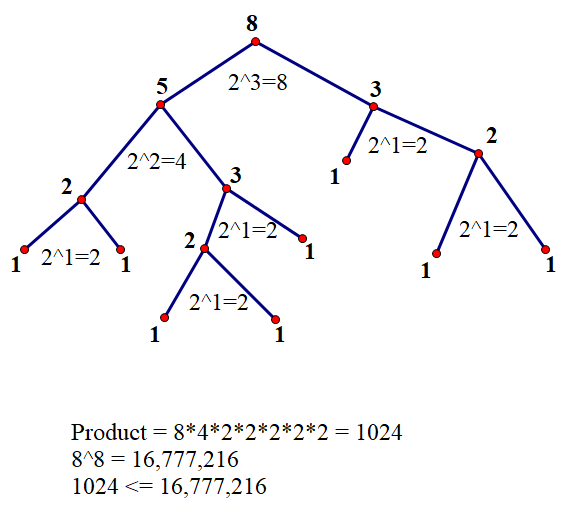
\includegraphics[scale=.75]{Homework/Images/induction.png}\end{center}

Prove using strong induction that no matter how you split the piles, the overall product you get is less than or equal to $n^ n$.

\textbf{Hint:} When there is only one stone, you cannot split the pile, and the process stops.

\begin{solution}

\end{solution}


\end{document}
